\chapter{Methodik und Anwendungszenarien} % (fold)
\label{cha:methodik}

In diesem Kapitel wird die Methodik vorgestellt, die zur Externalisierung von mentalen Modellen mit dem zu entwickelnden Werkzeug zur Anwendung kommt. Die Inhalte dieses Kapitels bauen auf den Ergebnissen der Kapitel \ref{cha:articulation_work}  und \ref{cha:mentale_modelle} auf. Die Anforderungen, die sich auf der hier vorgestellen Methodik ergeben, werden in Kapitel \ref{cha:anforderungen} identifiziert und in weiterer Folge in einem Werkzeug umgesetzt.

Basierend auf den Schlussfolgerungen, die \citet{Ifenthaler06} hinsichtlich der Eignung der beschriebenen Methoden zur Externalisierung von mentalen Modellen zieht, scheinen jene Ansätze, die auf der Bildung diagrammatischer Modelle basieren besser für die Unterstützung expliziter „Articulation Work“ geeignet zu sein als Methoden, die auf einer rein natürlichsprachlichen Repräsentation aufbauen. Dies liegt vor allem in der höheren Abstraktion begründet, die die externe Repräsentation als interindividuellen Ankerpunkt für Kommunikation besser geeignet macht. Dies deckt sich mit den Aussagen von  \citet{Sarini02}, \citet{Herrmann02}, \citet{Raposo04} oder \citet{Jorgensen04}, die aus Sicht von „Articulation Work“ für die Verwendung von (diagrammatischen) Modellen zur Unterstützung argumentieren.

Betrachtet man nun die beiden Vertreter der auf diagrammatischen Modellen aufbauenden Methoden -- Strukturlegetechniken und Concept Mapping --, so zeigt sich hinsichtlich der Eignung zum Unterstützung von „Articulation Work“ kein eindeutiger Vorteil für eine der beiden Methoden. Vielmehr weisen beide in diesem Kontext Vor- und Nachteile auf. Hier wird deshalb versucht, die Vorteile von Strukturlegetechniken -- im Wesentlichen die Unmittelbarkeit der physischen Repräsentation -- mit jenen von Concept Mapping -- der Flexibilität der Modellierung sowie der Möglichkeit der Unterstützung des Modellierungsprozesses durch Computersysteme -- zu vereinen.

Dabei wird auf das für „Articulation Work“ besser geeignete methodische Vorgehen von „Concept Mapping“ zurückgegriffen, während die Modellierungsumgebung an das Setting von „Strukturlegetechniken“ angepasst wird.

\section{Durchführungsrahmen} % (fold)
\label{sec:durchführungsrahmen}

Der Rahmen, in explizite „Articulation Work“ mit Unterstützung von externalisierten Modellen durchgeführt wird, ist an den Aufbau von Strukturlegetechniken angelehnt. Eine wesentliche Eigenschaft ist hierbei die physische Modellierungsoberfläche, auf der das Modell mittels real vorhandener und unmittelbar manipulierbaren Elementen aufgebaut wird. 

Im Sinne der Abstimmung unterschiedlicher Sichten muss eine kooperative, nicht exklusive Manipulierbarkeit des Modells gewährleistet sein. Das Modell selbst ist -- orientiert an der Offenheit der Repräsentation bei „Concept Mapping“ -- weder in der Art der Elemente noch der Beziehungen eingeschränkt. 

Hinsichtlich des Durchführungsrahmen ist auch die Notwendigkeit des Einsatzes einer Person zu diskutieren, die den Externalisierungsprozess anleitet und steuernd in diesen eingreift. Die Dialog-Konsens-Methode, die im Rahmen von Strukturlegetechniken zur Anwendung kommt, sieht die Rolle eines Untersuchungsleiters vor, der den Ablauf der Externalisierung strukturell anleitet. Inhaltlich hat der Untersuchungsleiter jedoch keine neutrale Rolle inne, sondern tritt im Rahmen des Dialog-Konsens-Prozesses in Interaktion mit der externalisierenden Person. Ziel des Untersuchungsleiters ist es, das mentale Modell der externalisierenden Person zu erschließen und zu verstehen. In kooperativen Situationen (die von der Dialog-Konsens-Methode nach \citep{Scheele88} nicht explizit berücksichtigt werden), wo gegenseitiges Verständnis erreicht werden muss, wechselt demnach die Rolle des Untersuchungsleiters inhaltlich gesehen dynamisch. 

Aus Sicht der Prozesssteuerung kann zu diesem Zeitpunkt nicht entschieden werden, ob ein Untersuchungsleiter benötigt wird oder nicht. Bei Strukturlegetechniken beschränkt sich dessen Aufgabe auf die Sicherstellung der Fokussierung der beteiligten Personen auf die jeweilige Aufgabe. Im Rahmen der Concept Mapping Methode ist ein intervenierender Untersuchungsleiter nicht vorgesehen. Im Rahmen der empirischen Erhebung (siehe Kapitel XY) wird untersucht, ob diese Rolle bei der Anwendung des hier vorgeschlagenen Werkzeugs notwendig ist oder unbesetzt bleiben kann. 

% subsection durchführungsrahmen (end)

\section{Vorgehen} % (fold)
\label{sub:vorgehen}

Sowohl im Bereich der Strukturlegetechniken als auch im „Concept Mapping“ wird vorgeschlagen, den initialen Modellierungsprozess in zwei Phasen -- Konzeptsammlung und Konzeptstrukturierung -- zu teilen und in der Folge das Modell iterativ solange zu verändern bzw. zu erweitern, bis alle Beteiligten mit der Lösung zufrieden sind (im Bereich der Strukturlegetechniken wird die als „Dialog-Konsens“ bezeichnet, im „Concept Mapping“ spricht man von „Revisions“ des Modells, die erstellt werden müssen). Beide Abläufe sind abstrahiert in Abbildung \ref{fig:img_MentaleModelle_slt_cm} dargestellt.

\begin{figure}[htbp]
	\centering
		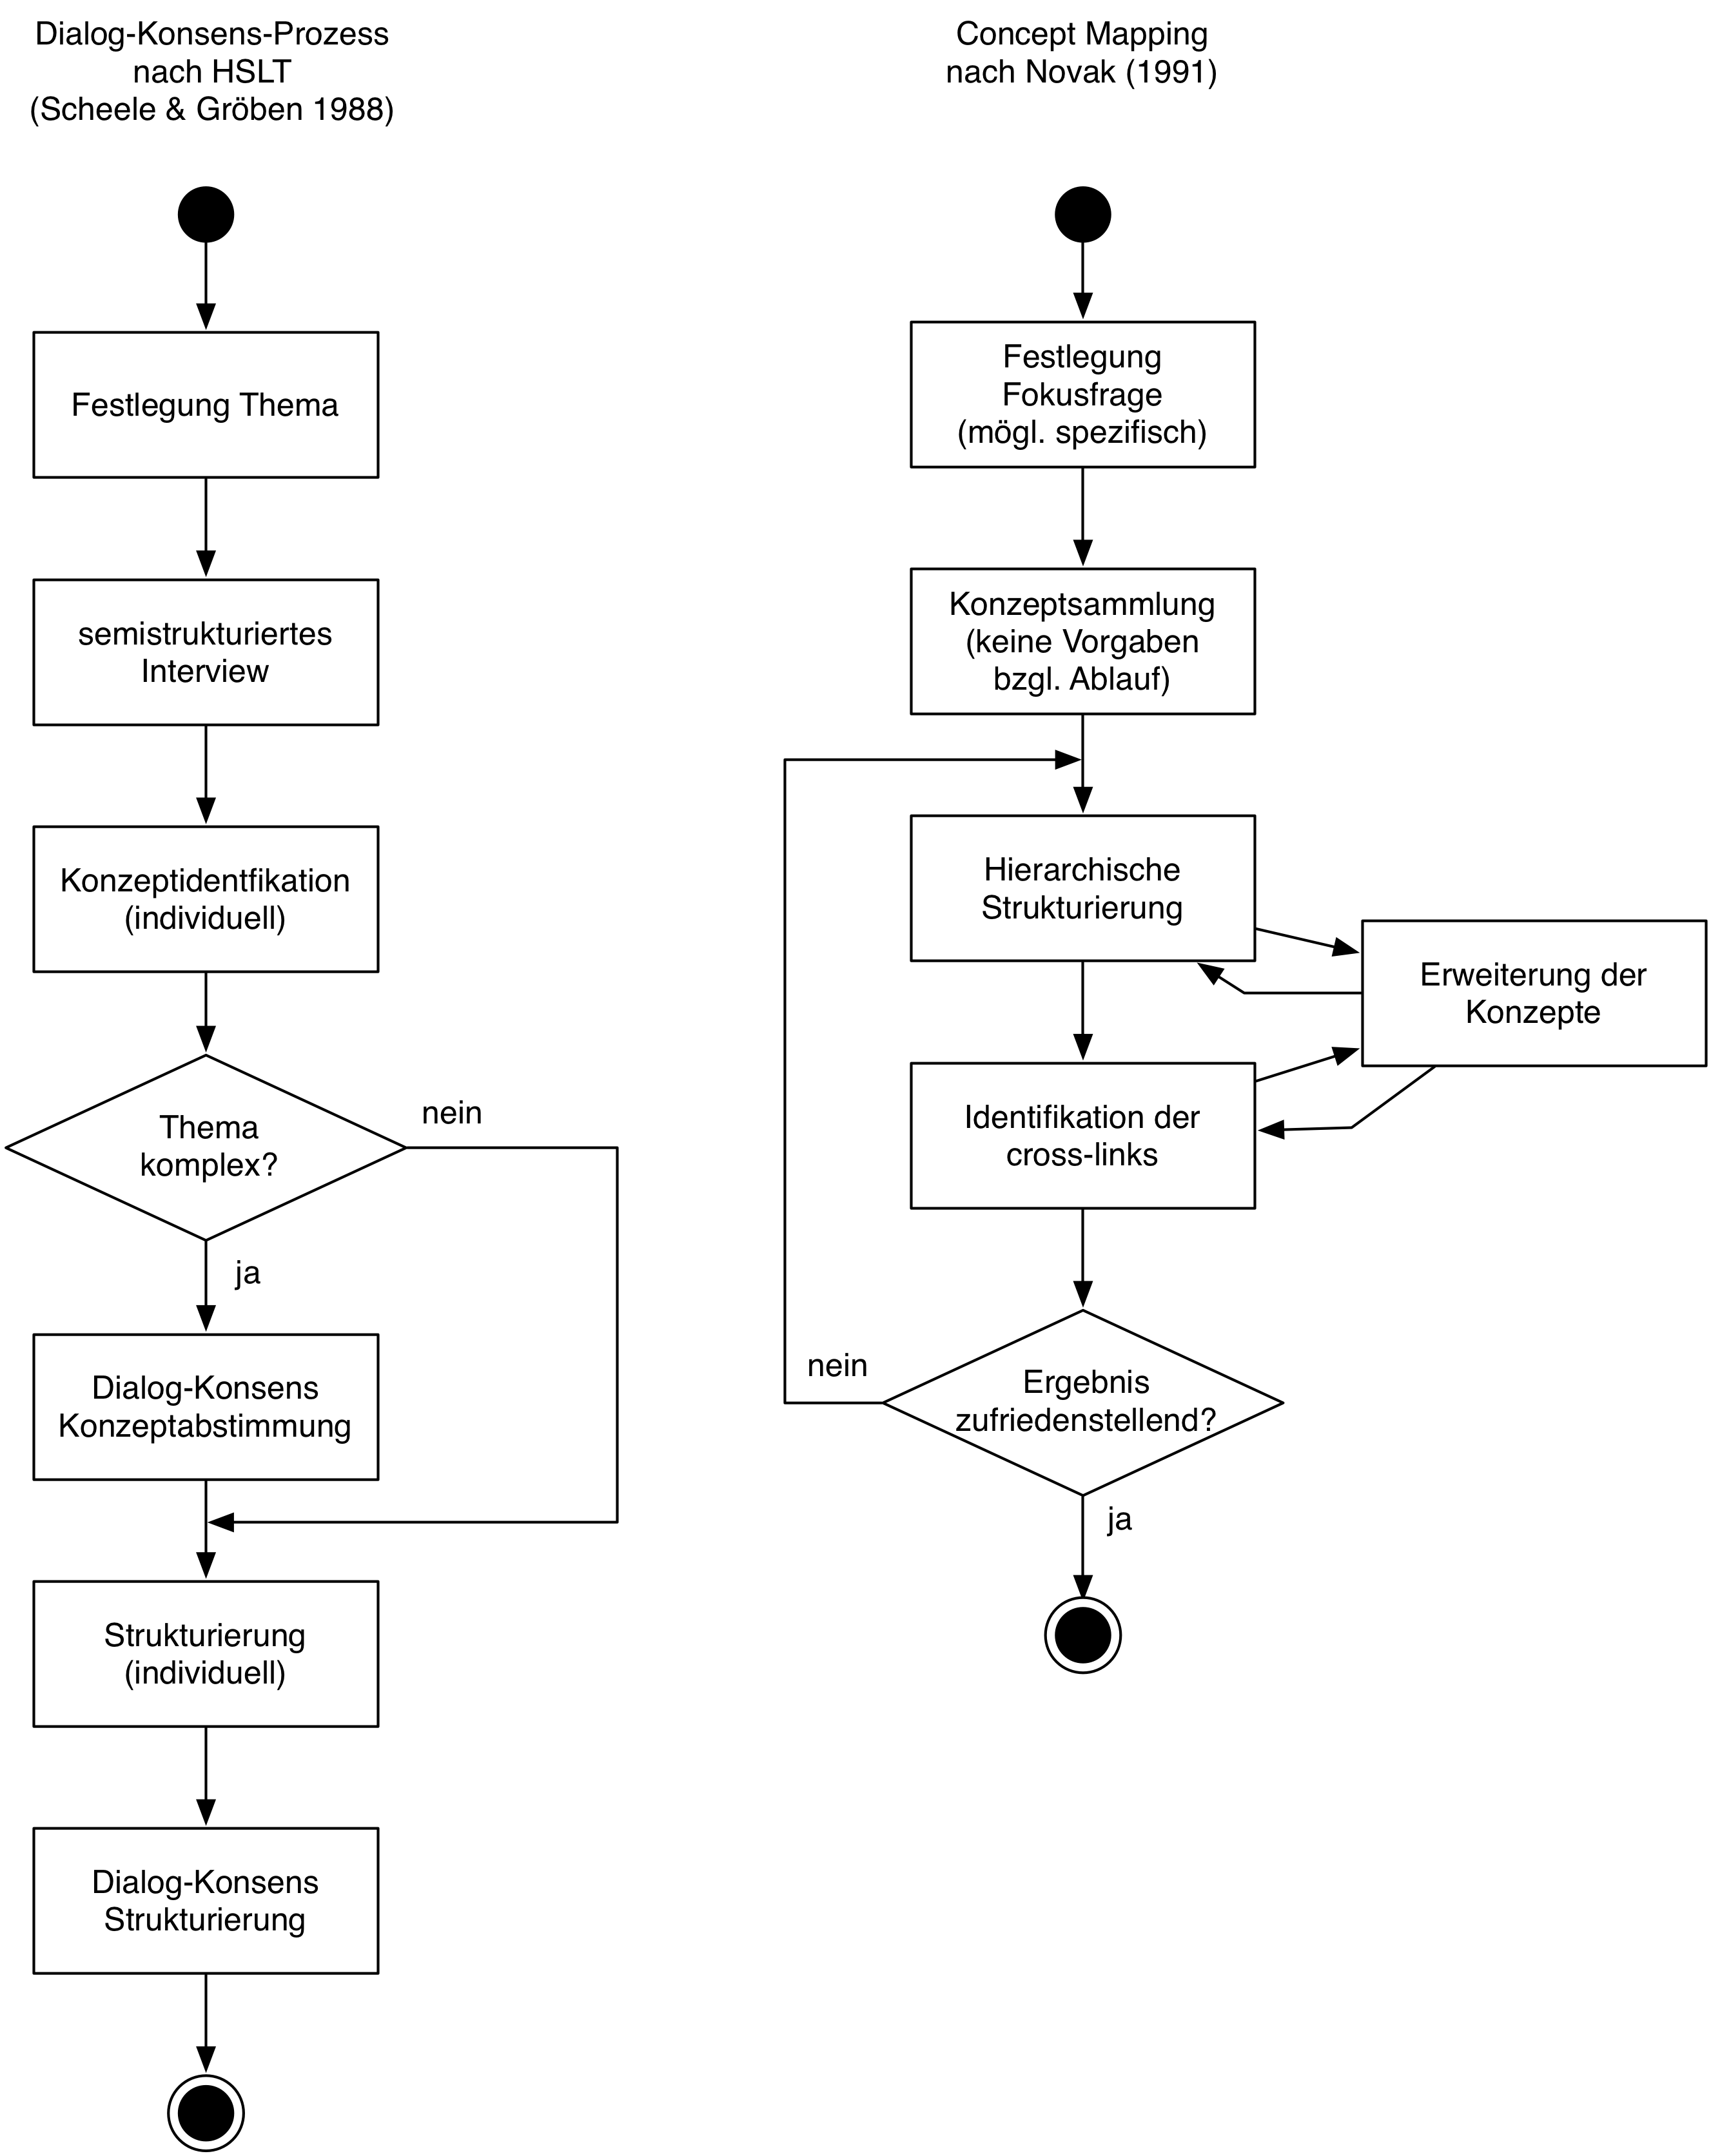
\includegraphics[width=\textwidth]{img/MentaleModelle/slt_cm.png}
	\caption{Externalisierung mentaler Modelle mittels Strukturlegetechniken und Concept Mapping}
	\label{fig:img_MentaleModelle_slt_cm}
\end{figure}

Das „Dialog-Konsens“-Vorgehen nach \citet{Scheele88} ist stark reglementiert und in den einzelnen Schritten mit definierten Methoden bzw. Vorgehensvorschriften hinterlegt. Die im Rahmen von „Concept Mapping“ vorgeschlagene Methode ist hier offener und erscheint damit für die Anwendung im Rahmen von „expliziter Articulation Work“ besser geeignet. Dies liegt am eher informellen Durchführungsrahmen von „expliziter Articulation Work“ begründet, deren Ausgestaltung individuell verschieden ist und zwischen den Beteiligten (im gängigsten Fall implizit) ausgehandelt wird. Ziel ist hier, den Artikulations-Prozess zu unterstützen und nicht, ihn zu formalisieren und in vorgegebene Ablauf-Grenzen zu pressen. 

Auch die zweiphasige Durchführung des Modellierungsprozesses muss unter diesem Gesichtspunkt hinterfragt werden. Die Unterteilung in zwei Phasen erscheint bei der Beschreibung von konzeptionellen Modellen sinnvoll. Begründet liegt dies in der Vielfalt möglicher Strukturierierungsvarianten bei dieser Art von Modellen. Im Gegensatz dazu ist die zweistufige Abhandlung der Externalisierung bei Modellen von Abläufen nur bedingt sinnvoll, da Aktivitäts-Konzepte im Normalfall bereits in deren kausalen Abfolge externalisiert und dann bzw. parallel mit zusätzlichen Konzepten hinterlegt werden. Diese Form von Modellen ist bei der Abstimmung von Arbeit gängig, wird aber weder bei Concept Mapping noch bei Strukturlegetechniken explizit angesprochen. Insofern ist die explizite Durchführung der ersten Phase -- also der Konzeptsammung -- als optional anzusehen. Im Sinne der Methode zur Erstellung von Concept Maps nach /citep{Novak06} werden Konzeptsammlungs-Phasen in den iterativen Modellverfeinerungsprozess eingeflochten, wenn dies in der Situation als notwendig erscheint.

Die einzelnen Schritte, die bei der Anwendung des Werkzeugs zur Anwendung kommen, sind im Einzelnen:
\begin{itemize}
 \item Einschulung
 \item Konzeptsammlung 
 \item Konzeptstrukturierung
 \item Restrukturierung
\end{itemize}

Diese Aufzählung gibt keine Reihenfolge der durchzuführenden Schritte vor. Vielmehr sind die einzelnen Blöcke als Module zu sehen, die je nach Anwendungsfall zu einem beliebigen Zeitpunkt im Externalisierungsprozess (auch mehrfach) zur Anwendung kommen oder auch entfallen können. Im Folgenden wird die Durchführung der einzelnen Schritte kurz umrissen und angegeben, in welchen Situationen deren Einsatz angemessen bzw. notwendig erscheint.

\subsection{Einschulung}

\subsection{Konzeptsammlung}

\subsection{Konzeptstrukturierung}

\subsection{Restrukturierung}
% section vorgehen (end)

\section{Anwendungsszenarien}

Prototypische Zusammenstellungen der Vorgehensblöcke je nach Setting der Abstimmung mentaler Modelle.

\begin{itemize}
 \item Verfeinerung individueller mentaler Modelle (rein indiv.)
 \item Wissenstransfer (1:n)
 \item Abstimmung individueller mentaler Modelle (indiv -> koop.)
 \item Aushandlung individueller mentaler Modelle (von Beginn an koop.)
\end{itemize}




% chapter methodik (end)